\section{Methodology}

This section describes some of the theory and methods involved in this work. Firstly, the governing equations of the numerical model are discussed in section \ref{subsec:LTE}. We then provide analytical expressions for the degree-2 tidal potential in section \ref{subsec:pot}. Following this, descriptions of the discretisation and numerical scheme are outlined in section \ref{subsec:model}, with a summary of the simulations ran in section \ref{subsec:param}.

\subsection{Laplace Tidal Equations \label{subsec:LTE}}

The equations of motion and mass conservation that describe ocean flow in the shallow water limit are known as the Laplace Tidal Equations (LTEs) \citep{lamb1932hydrodynamics}. The main assumption leading to this set of equations is that radial (vertical) ocean flow is negligible when compared to lateral flow, reducing the problem to two dimensions. This is indeed a good approximation for the Earth, where lateral flow length scales span much greater distances than the depth of the ocean. The conservation of mass (eq. \ref{eq:mass}) and momentum (eq. \ref{eq:mom}) that make up the LTEs, including both Rayleigh and bottom friction, are given as \citep{sears1995tidal,tyler2008strong,matsuyama2014tidal}:

%Adds vertical space between equations
%\setlength{\jot}{8pt}
%environment centres all equations

\vspace{-0.5cm}
\begin{gather}
\partial_t \eta + \nabla \cdot \left(h \bm{u}\right) = 0\, , \label{eq:mass}\\
\begin{aligned} 
\partial_t \bm{u} + 2 \bm{\Omega} \times \bm{u} + \alpha\bm{u} + \frac{c_D}{h} \left|\bm{u}\right| \bm{u}  + g \nabla \eta \\ = (1 + k_2 - h_2) \nabla U_2 \, . \label{eq:mom}\\
\end{aligned} 
\end{gather}

Equation \ref{eq:mass} consists of two terms. The first is the time rate of change of vertical sea surface displacement, $\eta$, about some equilibrium level, $h_0$, where the total ocean thickness, $h = h_0 + \eta$. The second term represents the divergence of the ocean depth multiplied by the surface velocity vector, $\bm{u} \equiv (u, v)$, where $u$ and $v$ are the eastward and northward velocity components, respectively.

The term on the right hand side of Equation \ref{eq:mom} is an applied force per unit mass. $\nabla U_2$ is the gradient of the degree-2 tide raising potential, discussed in section \ref{subsec:pot}. It is multiplied by Love's reduction factor, $1 + k_2 - h_2$. Love's first number, $k_2$, is a proportionality constant accounting for the additional tidal potential due to the elastic redistribution of mass on the satellite. $h_2$, the second Love number, accounts for the tidal potential arising from solid body surface displacement of the satellite \citep{love1911some}.

The time derivative of velocity is the first term on the left hand side of the momentum equation (eq. \ref{eq:mom}). It is balanced by four force per unit mass terms on the left hand side. The first of these terms is the coriolis acceleration, where $\bm{\Omega}$ is the satellite's rotational angular velocity vector. Rayleigh and bottom friction are described in the next two terms, where $\alpha$ and $c_D$ are the Rayliegh (linear) and bottom (quadratic) friction coefficients, respectively \citep{sears1995tidal,chen2013tidal}. The last term on the left hand side of Equation \ref{eq:mom} is the gravitational restoring acceleration per unit mass. It acts to restore changes in sea surface displacement about the undisturbed ocean depth, $h_0$.

\subsection{Tidal Potential \label{subsec:pot}}

Finite eccentricity and obliquity cause libration of the satellite's tidal bulge in longitude and latitude, respectively. It is this libration that primarily induces ocean flow. We therefore find it convenient to split the full degree two tidal potential into two main components, the eccentricity and obliquity tides:
\begin{align}
U_2 &= U_{ecc} + U_{obliq}\, . \label{eq:U_2}
\end{align}
The eccentricity and obliquity tide can be expressed as \citep{tobie2005tidal,tyler2011tidal,matsuyama2014tidal},
\begin{multline}
U_{ecc} = \Omega^2 r^2 e \left\lbrace - \frac{3}{2} P_{20}\left(\cos\theta\right) \cos \left(\Omega t \right) + \frac{1}{8} P_{22}\left( \cos\theta\right) \right. \\ 
\times \left. \vphantom{\frac{1}{8}} \left[7 \cos \left(2 \phi - \Omega t \right) - \cos \left(2 \phi + \Omega t\right) \right] \right\rbrace, \label{eq:U_ecc}
\end{multline} and,
\begin{multline}
U_{obliq} = \frac{1}{2}\Omega^2 r^2 \theta_0 P_{21}\left(\cos\theta\right)\\
\times \left[ \cos \left(\phi - \Omega t \right) - \cos \left( \phi + \Omega t\right) \right] \, ,\label{eq:U_obliq}
\end{multline}
where $r$ is the satellite's radius, $e$ is its eccentricity, and $\theta_0$ is the obliquity in radians. Co-latitude and longitude are given as $\theta$ and $\phi$ respectively. $P_{lm}$ represents the associated Legendre function of degree $l$ and order $m$. The eccentricity tide can be further split into the two terms on the right hand side of Equation \ref{eq:U_ecc}. These terms represent the eccentricity-radial ($U_{20}$) and eccentricity-libration ($U_{22}$) tides respectively, as described by \citet{tyler2011tidal}. We can therefore rewrite equation \ref{eq:U_2} as $U_2 = U_{20} + U_{21} + U_{22}$.

The derivatives of equations \ref{eq:U_ecc} and \ref{eq:U_obliq}, required to solve the LTE, are given in the appendix.

\subsection{Numerical Model \label{subsec:model}}

In this section we outline our two dimensional, finite difference computational fluid dynamics (CFD) model, known as Ocean Dissipation in Icy Satellites (ODIS). In its current form, ODIS is based extensively on the models discussed in and developed by \citet{zahel1973diurnalk,zahel1978influence} and \citet{sears1994tidal,sears1995tidal}. Firstly, we provide a description of the numerical grid. We then give an overview of the finite difference scheme itself, before summarising and illustrating limitations of the finite difference scheme and grid choice.

\subsubsection{Discretized Grid \label{subsec:grid}}

\begin{figure*}[t]
\centering
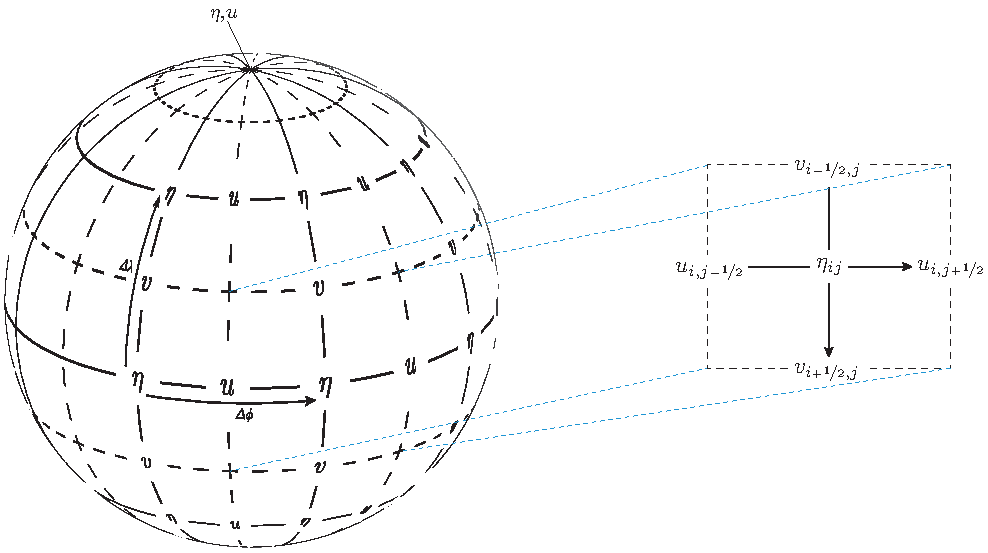
\includegraphics[width=0.8\linewidth]{Figures/GridDiagram}
\caption{The staggered grid structure used in ODIS. A single cell is show on the right of the figure, where surface displacement, $\eta$, represents a cell centered quantity. $u$ velocity nodes are staggered eastward of $\eta$, whereas $v$ velocity nodes are staggered southwards. Both $u$ and $v$ are defined at the cell walls. Lines of meridian merge to singularities at the poles, where both a single $u$ and $\eta$ point are stored.\label{fig:grid}}
\end{figure*}

We employ a fixed latitude-longitude grid for our numerical simulations, defined in a spherical coordinate system. The grid is constructed in a staggered manner, meaning that velocity nodes are placed to the east and south of their parent displacement nodes. This is illustrated in Figure \ref{fig:grid}, where we define $u$ and $v$ as the eastward and northward velocity components, respectively. $\Delta \lambda$ is the grid spacing in latitude, whereas $\Delta \phi$ is the grid spacing in longitude. A staggered approach is reasonably common in CFD problems as it avoids numerical oscillations that grow in the solution by calculating derivatives \textit{between} grid nodes rather than over them. This is discussed further in section \ref{subsec:fd_expan}.

As is clear from Figure \ref{fig:grid}, lines of meridian all converge to single points at either pole. As a result, the model is forced to go from $m$ points immediately surrounding the pole, to merely a single point at either pole. Accordingly, both single values of $\eta$ and $u$ are stored at each pole. This approach slightly differs from \citet{sears1995tidal}, whom stored only a single $\eta$ value at the poles.

ODIS stores three separate 2D arrays for $\eta$, $u$ and $v$. They are accessed in a parent-child configuration, whereby the velocity nodes immediately east and south of a displacement node are the children to their parent $\eta$. Both $u$ and $v$ at the southern and eastern walls of the cell in Figure \ref{fig:grid} are children to the central $\eta$ node. This is of little importance to the model's computations, but does lend some insight into the infrastructure of ODIS.

\subsubsection{Finite Difference Expansions \label{subsec:fd_expan}}

In order to solve the LTEs, we expand equations \ref{eq:mass} and \ref{eq:mom} in a semi-implicit finite difference scheme in spherical coordinates \citep{sears1995tidal}. By expanding $\bm{u}$ into its components, the momentum equation becomes,

\vspace{-0.6cm}
\begin{multline}
u_{ij}^{t+1} \approx  \left[ \,2 \Omega \bar{v}_{ij} \sin{\lambda_i} \vphantom{\frac{c_D}{h}\sqrt{\left(u_{ij}^{t}\right)^2}} - \alpha u_{ij}^{t} \right. \\ 
- \frac{c_D}{h}\sqrt{\left(u_{ij}^{t}\right)^2 + \left(\bar{v}_{ij}^{t}\right)^2}\cdot\left(u_{ij}^{t}\right)^2 - \frac{g}{R \cos{\lambda_i}} \frac{\partial \eta_{ij}^{t}}{\partial \phi_j} \\  
+ \left.\left(1 + k_2 - h_2\right) \frac{1}{R \cos{\lambda_i}} \frac{\partial U_{2,ij}^{t}}{\partial \phi_j} \right]  \Delta t + u_{ij}^{t} \, , \label{eq:momu_fd}
\end{multline}
\vspace{-0.6cm}
\begin{multline}
v_{ij}^{t+1} \approx  \left[ \,-2 \Omega \bar{u}_{ij} \sin{\lambda_i} \vphantom{\frac{c_D}{h}\sqrt{\left(u_{ij}^{t}\right)^2}} - \alpha v_{ij}^{t} \right. \\ 
- \frac{c_D}{h}\sqrt{\left(\bar{u}_{ij}^{t}\right)^2 + \left(v_{ij}^{t}\right)^2}\cdot\left(v_{ij}^{t}\right)^2 - \frac{g}{R} \frac{\partial \eta_{ij}^{t}}{\partial \lambda_i} \\  
+ \left.\left(1 + k_2 - h_2\right) \frac{1}{R} \frac{\partial U_{2,ij}^{t}}{\partial \lambda_i} \right]  \Delta t + v_{ij}^{t} \, , \label{eq:momv_fd}
\end{multline}

\noindent and the mass conservation equation becomes, 
\begin{equation}
\eta_{ij}^{t+1} \approx 
-\frac{h}{R \cos{\lambda_i}}\left(
\frac{\partial \left(v_{ij}^{t+1} \cos{\lambda_i}\right)}{\partial	\lambda_i}  
+\frac{\partial u_{ij}^{t+1}}{\partial	\phi_j}\right)
\Delta t
+ \eta_{ij}^{t}\, . \label{eq:mass_fd}
\end{equation}

Latitude and longitude are denoted by $\lambda$ and $\phi$ respectively. $i$ and $j$ represent the $i\text{th}$ and $j\text{th}$ latitude and longitude nodes within the grid. The time index is given by $t$, and $\Delta t$ represents the time-step. Overbars correspond to averages, a necessity given the staggered nature of the grid.

All derivatives of the degree-2 tidal potential (equations \ref{eq:U_ecc} and \ref{eq:U_obliq}) have analytical solutions, and thus do not require further finite difference expansions. These derivatives are given in the appendix. Derivatives of all other quantities, however, do require further expansion. The expansions take the general form of either,

\begin{align}
\frac{\partial w_{ij}}{\partial \lambda} &\approx \frac{w_{i+\nicefrac{1}{2},j} - w_{i-\nicefrac{1}{2},j}}{\Delta \lambda} \, , \label{eq:gen1}
\shortintertext{or, }
\frac{\partial w_{ij}}{\partial \phi} &\approx \frac{w_{i,j+\nicefrac{1}{2}} - w_{i,j-\nicefrac{1}{2}}}{\Delta \phi} \, , \label{eq:gen2}
\end{align}

\noindent where $w$ represents $u$, $v$ or $\eta$.

Examining equations \ref{eq:gen1} and \ref{eq:gen2} reveals that each derivative is evaluated halfway between the nodes where $w$ is stored. Consequently, any derivative of $w$ is calculated half way between $w$ nodes; a position held by a different variable because the grid is staggered. For example, $\partial_\phi u_{ij}$ is always evaluated at the position held by $\eta_{ij}$ as $u_{i,j-\nicefrac{1}{2}}$ and $u_{i,j+\nicefrac{1}{2}}$ lie to the left and right of $\eta_{ij}$,  respectively. This is shown in Figure \ref{fig:grid}.

\subsubsection{Numerical Scheme}

ODIS begins its calculations by (1) determining the mass of each volume element in the initial ocean assuming an undisturbed ocean of depth $h_0$. With the mass calculated in each cell, it is then possible to find the dissipated energy in the system.

The next step in the numerical integration is to calculate $\nabla U_2$ across all $u$ and $v$ grid points (2). This gives the initial force per unit mass experienced by a fluid element in the model domain.

Once the tidal acceleration is known, ODIS directly calculates $u$ and $v$ over the grid by solving equations \ref{eq:momu_fd} and \ref{eq:momv_fd} (3). This step is purely explicit as $u$ and $v$ depend only on information from the previous time step, $t$. Following this, $\eta$ is then updated using the new velocity values (4). In contrast to the velocity calculations, this step is semi-implicit as it relies on values from both the current and previous time steps, as shown in Equation \ref{eq:mass_fd}.

After solutions for $u$, $v$, and $\eta$ are found at the new time step, $t+1$, the energy calculations begin (5). For Rayleigh friction, ODIS calculates and stores global dissipated energy flux as,
\begin{equation}
F_{\alpha}^{t+1} = \frac{1}{4 \pi R^2 }\sum_{i=1}^{n} \sum_{j=1}^{m} \alpha M_{ij} \left[\left(u_{ij}^{t+1}\right)^2 + \left(v_{ij}^{t+1}\right)^2\right] \, , \label{eq:E_alpha}
\end{equation}

for $n$ and $m$ grid points in latitude and longitude, respectively. 

The summed terms in Equation \ref{eq:E_alpha} give the total dissipated energy in the system across the current time step, for each cell of mass $M$. The factor in front of the summations then averages this quantity over the satellite's surface area giving $F_{\alpha}$ in watts per square metre. For bottom friction the equivalent expression is,
\begin{equation}
F_{c_D}^{t+1} = \frac{1}{4 \pi h R^2 }\sum_{i=1}^{n} \sum_{j=1}^{m} c_D M_{ij} \left[\left(u_{ij}^{t+1}\right)^2 + \left(v_{ij}^{t+1}\right)^2\right]^{\nicefrac{3}{2}}\, . \label{eq:E_cd}
\end{equation}
Details of these derivations are discussed in the appendix.

Every time step the previous calculations (2-5) are repeated, beginning from determining $\nabla U_2$. Finally, at the end of each orbit, $F_\alpha$ or $F_{c_D}$ is summed and averaged over the orbital period (6). This gives the orbitally averaged surface heat flux due to tidal dissipation for Rayleigh friction,
\begin{align}
\left\langle F_\alpha \right\rangle_{orbit} &= \sum_{t=0}^{p} F_{\alpha}^{t}  \, , \label{eq:E_alpha_orbit}
\shortintertext{and bottom friction,}
\left\langle F_{c_D} \right\rangle_{orbit} &= \sum_{t=0}^{p} F_{c_D}^{t}  \, , . \label{eq:E_cd_orbit}
\end{align}

where $p = \nicefrac{T}{\Delta t}$, the total number of time steps in the orbital period, $T$. These expressions are consistent with \citep{sears1995tidal}.

\begin{figure}[!t]\centering
\begin{subfigure}{\linewidth}
\centering
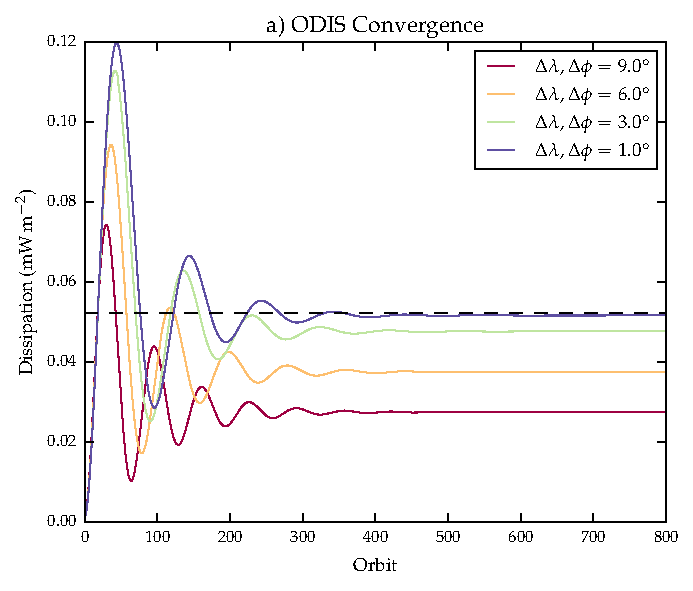
\includegraphics[width=0.95\linewidth]{Figures/res_test}
\subcaption{\label{fig:conv_a}}
\end{subfigure}\vspace*{-0.7cm}
\begin{subfigure}{\linewidth}
\centering
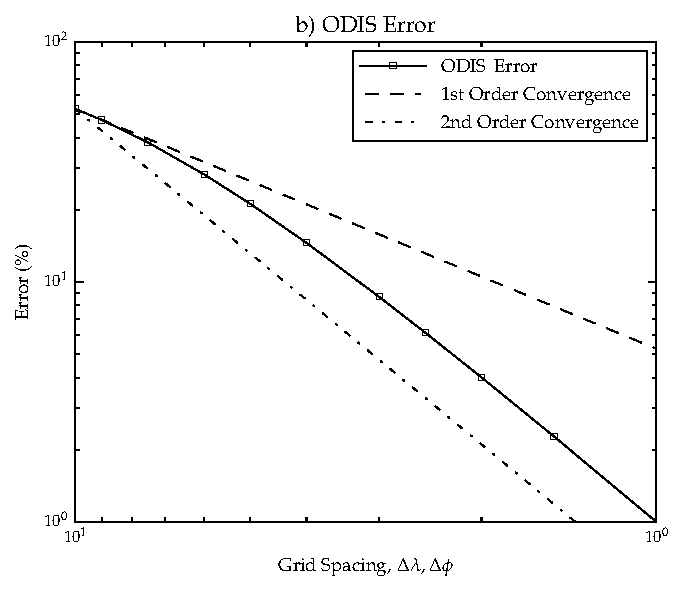
\includegraphics[width=0.95\linewidth]{Figures/error}
\subcaption{\label{fig:conv_b}}
\end{subfigure}\vspace*{-0.7cm}
\caption{Convergence and error scaling as a function of grid resolution. Plot \ref{fig:conv_a} on the top shows the time evolution of dissipated energy at periapse. The solid line represents different grid resolutions, whereas the dashed line is the anlytically derived dissipated energy. After 500 - 600 orbits, startup oscillations in the solution begcome neglible and the solution has converged. Figure \ref{fig:conv_b} on the bottom shows the error between the numerical and analytical solutions with increasing resolution. The numerical solution falls between 1st and 2nd order convergence with increasing resolution. All simulations are for the obliquity tide using $h = 1 \, \si{\kilo\metre}$ and $\alpha = 10^{-8} \, \si{\per\second}$. \label{fig:conv}}
\end{figure}

Steps 2-6 are repeated until the model has converged into a periodic solution. Care must be taken when selecting convergence criteria. Simulations involving deep oceans and small friction coefficients will oscillate about their converged solution with periods of 10 - 100 orbits due to the large inertia associated with deep, poorly dissipative oceans (see Figure \ref{fig:conv_a}). These simulations clearly require longer run-time.


\subsubsection{Grid Limitations and Resolution Testing \label{subsubsec:grid_lim}}

As with any numerical solution there are errors associated with discretization of the problem into the model domain. We performed resolution testing across various ocean depths to determine how these errors scale with grid resolution. One of these tests is shown in Figure \ref{fig:conv}. The upper plot shows how the numerical time-averaged dissipated energy solution converges to a final value. As grid resolution is increased the numerical estimate converges to the analytically derived solution. The lower plot (Figure \ref{fig:conv_b}) shows the numerical error as a function of increasing resolution, indicating first to second order convergence in the numerical solution. Based on these resolution tests, all further simulations were ran for grid spacings of $\ang{2}$ in latitude and longitude. 

A natural issue arising from the choice of grid is the time step used. As described in section \ref{subsec:grid}, the fixed latitude-longitude grid causes meridian lines to converge at the poles. Nodes near each pole therefore have much smaller spatial separations than those at the equator. In order to satisfy the Courant-Friedrichs-Lewy (CFL) condition required for numerical stability, $\Delta t \lesssim 40 \si{\second}$ if $\Delta \lambda = \Delta \phi = 4^{\circ}$ \citep{arakawa1977computational,sears1995tidal}. This massive constraint on the time step is often referred to as the ``pole problem''. Several workarounds to ease the time step have been applied throughout the literature \citep{comblen2009finite}. For example, it is common to apply a Fourier filter to remove high wavenumber components of the solvable fields near the poles \citep{murray2002fourier}, or to use the spectral transform method as reviewed by \citet{swarztrauber1996spectral}. In this work, however, we apply none of these methods, and obey the CFL condition by selecting the appropriate time step for the model resolution.

\begin{figure}[!b]
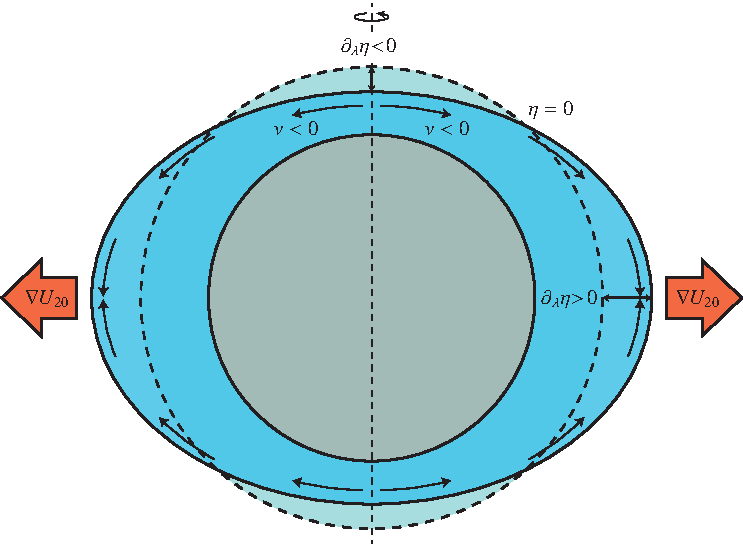
\includegraphics[width=\linewidth]{Figures/CoordProb}
\caption{Schematic representation of the ocean tide due to the eccentricity-radial tidal potential ($U_{20}$), at periapsis. Taking a derivative of $v$ across the north pole yields a null result in the spherical coordinate system, despite the clear mass divergence away from the poles leading to $\eta < 0$.\label{fig:coord_prob}}
\end{figure}

A more significant issue arises from the combined choice of coordinate system and grid structure. Nodes located directly at the poles become singularities in space, as the normal directions east and west used to define the velocity components become meaningless. Consider the northward velocity flow near the north pole under the eccentricity-radial tide, shown in Figure \ref{fig:coord_prob}. Conservation of mass and the formation of an equatorial bulge force flow to diverge away from the pole. In solving for the surface displacement node directly at $\lambda = 90^{\circ}$, we must take the derivative of $v$ across the pole (as in Equation \ref{eq:momv_fd}). As each $v$ node located either side of the pole has the same magnitude and, perhaps unintuitively, is orientated in the same direction (southwards), this derivative becomes zero. Longitudinal symmetry in $u$ causes the $u$ derivative from Equation \ref{eq:momu_fd} to be also zero. This forces surface displacement at the pole to zero as well. Yet, as there is divergence away from the pole, it is required that $\eta < 0$ to conserve mass. Clearly, the choice of coordinate system and grid do not permit such behaviour at the poles. 

To work around this problem, we employ first-order accurate one dimensional Euler interpolation for all $u$ and $\eta$ nodes located at the pole, avoiding the need to directly solve for these points. We then take the mean of the interpolated $\eta$ points and prescribe that as the polar value. The mean is not taken for $u$, as this reduces to zero around the pole due to cancellation of longitudinally symmetric positive and negative velocities.

\subsection{Model Setup and Parameters \label{subsec:param}}



All numerical results presented in the following section are for surface oceans on Titan and Enceladus. Titan is an appropriate benchmark for our numerical model because, as already discussed, much of the numerical scheme used in this work is described by \citet{sears1995tidal} who applied his model to Titan.

We first perform both semi-analytical and numerical simulations for Titan under the eccentricity and obliquity tides. For each tidal component 3381 simulations were run for \hbox{$h = 1 - 10^4 \, \si{\metre}$} and \hbox{$\alpha = 10^{-9} - 10^{-5} \, \si{\per\second}$}. The semi-analytical solution for the orbitally averaged surface heat flux was directly compared to the numerical values to reveal any inaccuracies in the numerical model across this parameter space. 

Following testing and verification of the numerical solutions for Rayleigh friction, ODIS was then run using only bottom friction for \hbox{$h = 1 - 10^4 \, \si{\metre}$} and \hbox{$c_D = 10^{-7} - 10^{-1} \, \si{\per\second}$}. These simulations were again run for both the eccentricity and obliquity tides, where 5037 simulations were run for each main tidal component. With results for both Rayleigh and bottom friction we were able to make comparisons about tidal dissipation under these two friction models. This process was then recreated for Enceladus assuming both Rayleigh and bottom friction. The model parameters used for both Titan and Enceladus are shown in Table \ref{tb:param}.

Numerically solving the LTEs to convergence is computationally an expensive process. As shown in Figure \ref{fig:conv_a}, convergence may only be reached after a significant amount of simulation time. The example given in Figure \ref{fig:conv_a} was run using initial conditions for an at rest, undisturbed ocean. To speed up convergence we employ the technique used by \citep{sears1995tidal}, whereby the final output of one simulation is used as the initial conditions for the next simulation. Upon completion, each running process will spawn one to two `child' simulations. These new process will in turn spawn there own `children' once they are complete. This logical way of solving over such a large parameter space helps to significantly reduce computational run time. Several tests were also ran to unsure that a given simulation would return converge to a single solution, regardless of initial conditions.

\begin{table}[!t]
\scriptsize
\centering
\begin{tabularx}{\linewidth}{p{1.8cm} p{2cm} p{1cm} p{1.2cm}}
 \toprule
Parameter & Description & Titan & Enceladus\\
 \midrule \midrule
$\Omega$ [$\times 10^{-5}$ \si{\radian\per\second}]	& angular velocity 		& $0.455$ & $5.31 $ \\
$r$ [\si{\kilo\metre}]				& satellite radius 		& $2574.7$ & $252.1$\\
$a$ [$\times 10^6$ \si{\kilo\metre}]				& semi-major axis 		& $1.221865$ & $0.238042$\\
$g$ [\si{\metre\per\second\squared}]		& surface gravity 		& $1.35$ & $0.11$\\
$e$ 								& eccentricity 			& $0.0288$ & $0.0044$\\
$-\theta_0$ [$^{\circ}$] 			& obliquity 			& $0.32$ & $0.0027$\\
$k_2$ 								& tidal Love number 	& $0.120$ & $0.0010$\\
$h_2$ 								& tidal Love number 	& $0.221$ & $0.0017$\\
 \bottomrule
\end{tabularx}
\caption{Model parameters used in all simulations presented here. All values are specific to Titan, and are taken from \citet{zebker2009size,chen2013tidal}.  \label{tb:param}}
\end{table}

\begin{figure*}[!t]
\begin{subfigure}{\linewidth}
\centering
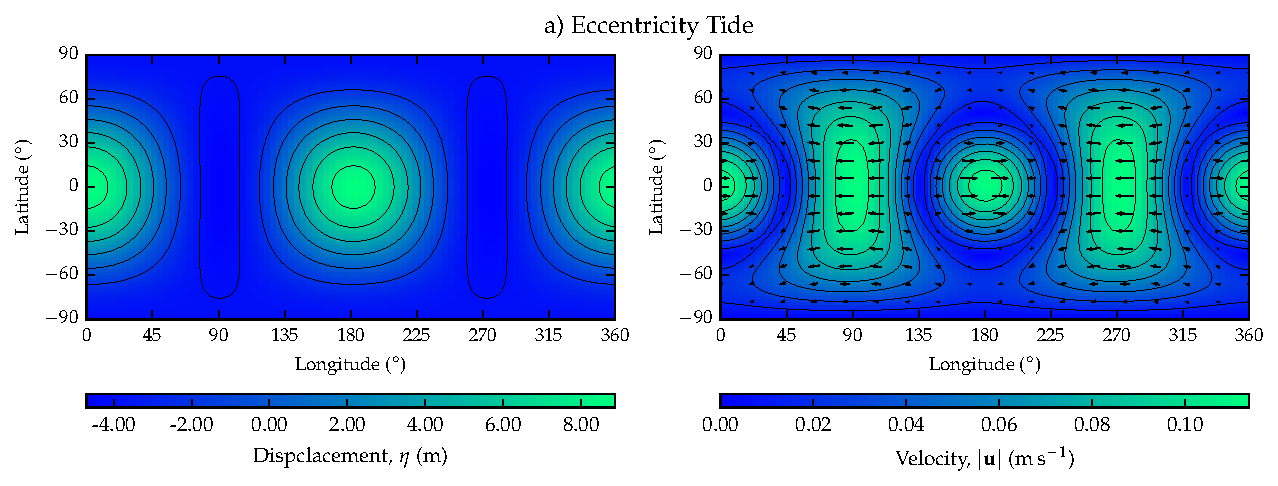
\includegraphics[width=0.8\linewidth]{Figures/Ecc_test}
\subcaption{\label{fig:LTE_a}}
\end{subfigure}\vspace*{-0.7cm}
\begin{subfigure}{\linewidth}
\centering
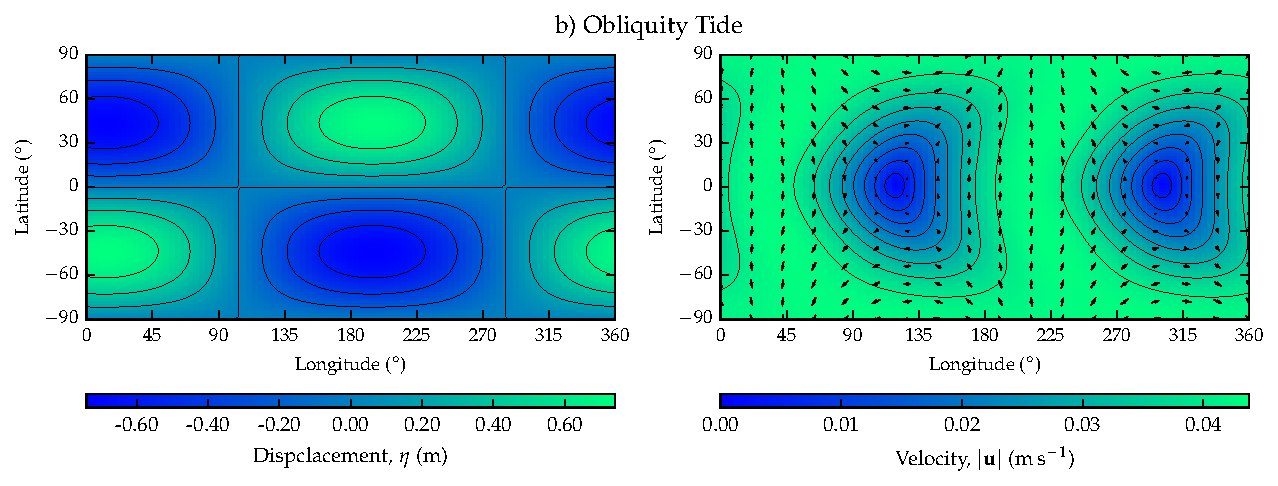
\includegraphics[width=0.8\linewidth]{Figures/Obliq_test}
\subcaption{\label{fig:LTE_b}}
\end{subfigure}\vspace*{-0.7cm}
\begin{subfigure}{\linewidth}
\centering
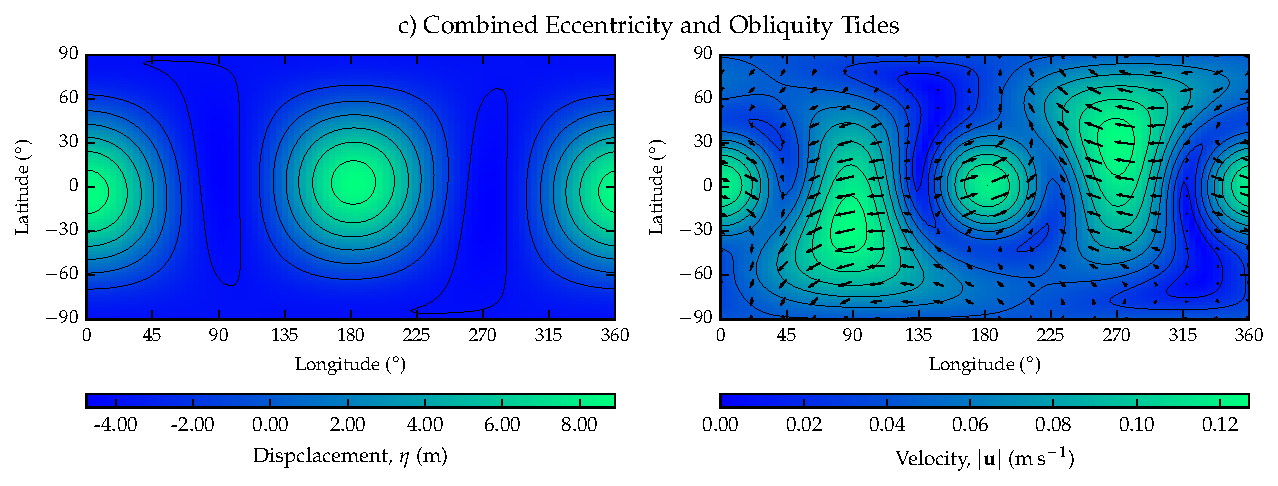
\includegraphics[width=0.8\linewidth]{Figures/Full_test}
\subcaption{\label{fig:LTE_c}}
\end{subfigure}\vspace*{-0.8cm}
\caption{Solutions to the LTE under the eccentricity (eq. \ref{eq:U_ecc}), obliquity (eq. \ref{eq:U_obliq}), and full tidal potential (eq. \ref{eq:U_2}) for Rayleigh friction. All figures shown are at periapsis for ocean parameters $h = 400 \, \si{\metre}$ and $\alpha = 2.28 \times 10^{-7} \, \si{\per\second}$. \label{fig:LTE_solns}}
\end{figure*}


